\documentclass{csse4400}

\usepackage{CJKutf8}
\usepackage{languages}

\title{Scalable Text-to-Speech}
\author{Brae Webb}
\date{Semester 1, 2022}

\begin{document}
\maketitle

\section*{Summary}
In this assignment, you will demonstrate your ability to \textsl{design},
\textsl{implement}, and \textsl{deploy} a web application that can process a high load,
i.e. a scalable application.
You will be asked to deploy a tool that accepts text input and generates synthesized speech output.
Specially you need to support:
\begin{itemize}
    \item Uploading and generating a large text input.
    \item Generating speech output while remaining responsive to the user.
    \item Access via a specified REST API for use by front-end interfaces.
\end{itemize}

Your service will be deployed to AWS and will undergo automated correctness and load-testing to ensure it meets the required scalability.

\section{Introduction}
Text-to-speech software supports accessibility,
enables smart-home devices,
and even breaks down language barriers.
Unfortunately, text-to-speech is computationally intensive.
While the technology has made great advances over the past few decades,
many open-source implementations are still inefficient.

\paragraph{Task}
For this assignment,
the University of Queensland is looking to convert all course content into speech.
This will support visually impaired students in their studies.
All course content from slack messages and blackboard announcements to text-books must be converted to speech.
You will be responsible for designing and implementing this service for use across the entire university.

\paragraph{Requirements}
As you might imagine,
blackboard announcements occur frequently and should be translated in almost real time.
While textbooks are set ahead of semester and may take several days to process.
The university will experience peaks of usage.
At the start of semester,
instructors many set textbooks which need to be processed.
The university will also experience usage lows over the summer holiday period when no translations will be required.
The university is not willing to pay for the resources required during start of semester all year round.
Your implementation must be able to scale dynamically based on the current amount of jobs to be processed.

% \section{Features}


\section{Interface}
Your service will be utilised by almost every system in the university.
It has been decided that every university services must support text-to-speech on the first Monday of semester two.
An interface specification has already been developed and distributed to existing service owners,
who are working hard to deliver support in their services.

You must implement this interface exactly as described,
the interface specification is available to all service owners online:
\url{https://csse6400.uqcloud.net/assessment/chatterbox}

\section{Submission}
Your final solution will be committed to a GitHub repository.
Committing to this repository will be disabled after \textbf{16:00 (AEST) on 6 May 2022} and the contents of the repository at this time will be taken as your submission.
The repository \textbf{must} contain everything required to successfully deploy your application.
You must include all of the following in the repository:
\begin{itemize}
  \item Your implementation of the service API, including the source code and a mechanism to build the service.%
  \footnote{If you are using external libraries, ensure that you pin the version to avoid external changes breaking your application.}
  \item Terraform code that can provision your service from a fresh AWS learner lab environment.
\end{itemize}

When deploying your application to mark,
we will follow rigid and reproducible steps.
We outline the steps here so that you may re-create the process yourself.

\begin{enumerate}
  \item Your Git repository will be checked out locally.
  \item AWS credentials will be copied into your repository in the top-level directory.
  \item The script \texttt{deploy.sh} in the top-level of the repository will be run.
  \item The \texttt{deploy.sh} script \textbf{must} create a file named \texttt{api.txt} which contains the URL where your API is deployed to.
  \item We will run automated load-testing on the URL provided in the \texttt{api.txt} file.
\end{enumerate}

\subsection{Tips}

\paragraph{Outputting an API URL}
Your Terraform code should produce a URL where you API can be accessed from.
A requirement is that this URL is stored to \texttt{api.txt}.
We recommend that you use the \texttt{local\_file} resource to accomplish this.

\begin{code}[language=terraform]{}
resource "local_file" "url" {
    content  = # some resource output here
    filename = "./api.txt"
}
\end{code}

\paragraph{Terraform apply in deploy script}
Your \texttt{deploy.sh} script must deploy without user interaction.
You run Terraform apply without prompting for configuration using the command:
\bash{terraform apply -auto-approve}

\paragraph{If something goes wrong}
Ideally, your infrastructure will be provisioned successfully but this may go wrong for a number of unforeseen reasons.
If something does go wrong during deployment,
teaching staff will refer to your \texttt{README.md} file to attempt to resolve the issue where possible.
Please ensure that your \texttt{README.md} documentation is of high quality to allow yourself the best chance for recovery.

\paragraph{Fresh AWS learner lab}
Your AWS learner lab can be reset using the reset button in the learner lab toolbar.
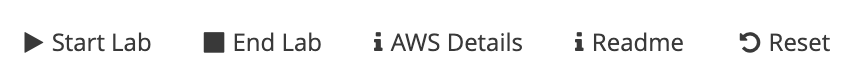
\includegraphics[width=\textwidth]{images/reset-button.png}
To ensure that you are not accidentally depending on anything specific to your learner lab environment,
we recommend that you reset your lab prior to final submission.
Note that resetting the lab can take a considerable amount of time,
in the order of hours,
so please do not do this at the last minute.

\paragraph{Deploying with Docker}
In this course,
you have been shown how to use Docker containers to deploy EC2 instances \cite{prac-week5}.
You may find it a pragmatic way to deploy your application in this assignment.
If you intend to deploy using Docker containers,
we recommend that you create a GitHub actions workflow
to build and publish your container to the GitHub container registry.
An example of this can be seen in the \link{todo-app}{https://github.com/CSSE6400/todo-app/blob/main/.github/workflows/backend.yml}.
Containers can then be deployed from a ghcr URL, e.g. \url{ghcr.io/csse6400/todo-app}.

\todo{This needs to be private \& needs to show how to login}

\paragraph{Unique S3 buckets}
You may find it helpful to use S3 buckets for this assignment.
It is important to be aware the the name of an S3 bucket has to be \textsl{globally} unique.
To avoid any deployment conflicts,
we recommend that you use the \texttt{random\_string} Terraform resource.
This allows you to generate a random string which can be appended to the S3 bucket name.

\begin{code}[language=terraform]{}
resource "random_string" "bucket-name" {
    length    = 16
    special   = false
    upper     = false
}

resource "aws_s3_bucket" "bucket" {
    bucket = "my-bucket-${random_string.bucket-name.result}"
}
\end{code}

\todo{S3 signed URLs}


\subsection{Fine Print}
You can reproduce our process for deploying your application using our \link{Docker image}{https://ghcr.io/CSSE6400/csse6400-cloud-testing}:
\codefile[language=docker]{Dockerfile}{deployment/Dockerfile}

\noindent
Our steps for deploying your infrastructure using this container are as follows,
\texttt{\$REPO} is the name of your repository,
\texttt{\$CREDENTIALS} is the path where we will store our AWS credentials:
\begin{code}[language=shell]{}
$ git clone git@github.com:CSSE6400/$REPO
$ cp $CREDENTIALS $REPO
$ docker run -v /var/run/docker.sock:/var/run/docker.sock -v $(pwd)/$REPO:/workspace csse6400-cloud-testing
$ cat api.txt # this will be used for load-testing
\end{code}

\noindent
Note that the Docker socket of the host has been mounted,
this enables running \texttt{docker} in the container.
This has been tested on MacOSX and Linux but might require WSL2 on Windows.

\section{Criteria}

\section{Academic Integrity}
As this is a higher-level course, you are expected to be familiar with the importance of academic integrity in general, and the details of UQ's rules.
If you need a reminder, review the \link{Academic Integrity Modules}{https://web.library.uq.edu.au/library-services/it/learnuq-blackboard-help/academic-integrity-modules}.
Submissions will be checked to ensure that the work submitted is not plagiarised.
If you have quoted or paraphrased any material from another source, it must be correctly \link{cited and referenced}{https://web.library.uq.edu.au/node/4221/2}.
Use the \link{IEEE referencing style}{https://libraryguides.vu.edu.au/ieeereferencing/gettingstarted} for citations and your bibliography.

Uncited or unreferenced material will be treated as not being your own work.
Extensive quotation or minor rephrasing of material from cited sources should be avoided.
Significant amounts of cited material from other sources, even if paraphrased, will be considered to be of no academic merit.
In all cases, any material that you cite must support the arguments and points that you are making in your presentation.

\bibliographystyle{ieeetr}
\bibliography{ours}

\end{document}